% mms-viscous.tex

\section{Method of manufactured solutions -- Viscous flow}
\label{mms-viscous-sec}
\index{source terms!user defined!example of use}\index{verification}
\index{Maxima!example of use}\index{verification}
\index{e3mpi.exe!example of use}\index{verification}
%
This extends the method of manufactured solutions 
as a code verification exercise to viscous flow.
If you thought that the user-defined source terms for 
the Euler case (Section\,\ref{mms-euler-sec}) were ugly,
the viscous terms are so bad we no longer look at them.
Here all of the source-term code is machine generated, 
principally by the Maxima computer algebra system and then 
with a bit of text processing by a Python script.

\begin{figure}[htbp]
\begin{center}
\mbox{
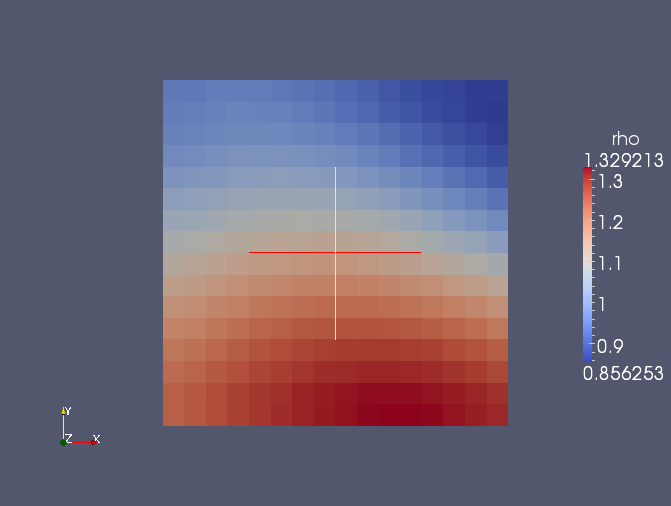
\includegraphics[width=0.5\textwidth]{../2D/mms/density-field-at-80ms.png}
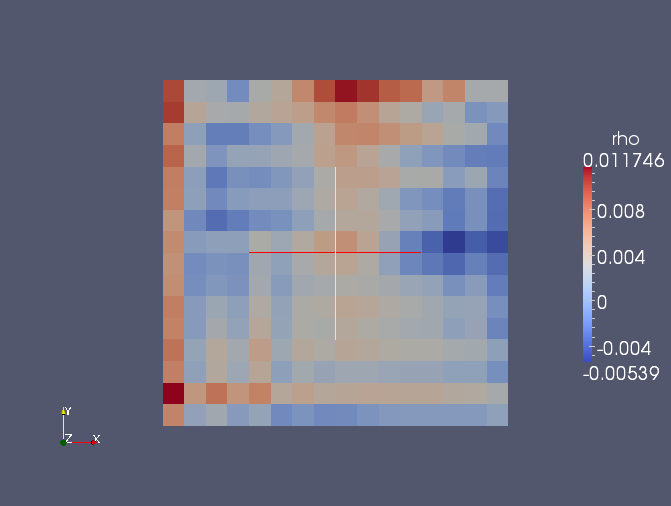
\includegraphics[width=0.5\textwidth]{../2D/mms/density-error-at-80ms.png}
}
\end{center}
\caption{Density and error-in-density fields for the steady-state solution for the
  viscous (case=2) Method of Manufactured Solutions.}
\label{mms-viscous-density-error-fig}
\end{figure}

\noindent
Note the smooth solution for the density field but the pattern of errors hinting
at the 4 blocks used in this simulation.
With respect to interior points in a block, the viscous terms are estimated 
with fewer data along the edges and at the corners.

\bigskip\noindent
Rowan might like to add his convergence plots here...

\newpage
\subsection{Input script (.py)}\index{boundary conditions!UserDefinedBC!example of use}
\topbar
\lstinputlisting[language={}]{../2D/mms/mms.py}
\bottombar

\newpage
\subsection{Boundary condition file (.lua)}
\topbar
\lstinputlisting[language={}]{../2D/mms/udf-bc.lua}
\bottombar

\newpage
\subsection{Source term file (.lua)}
%
The source terms are generated with the aid of the Maxima computer algebra system
and inserted into the following template.
The expressions for \texttt{fmass}, \texttt{fxmom}, \texttt{fymom}, and \texttt{fe}
turn out to be 10, 23, 23 and 124 lines of 80-column text.\\
\topbar
\lstinputlisting[language={}]{../2D/mms/udf-source-template.lua}
\bottombar

\bigskip
\noindent
The Maxima script to do the real work is:\\
\topbar
\lstinputlisting[language={}]{../2D/mms/make_source_terms.mac}
\bottombar

\bigskip
\noindent
And the generated Fortran90 code is translated into Lua code with the Python script:\\
\topbar
\lstinputlisting[language={}]{../2D/mms/f90_to_lua.py}
\bottombar

\newpage
\noindent
Also, a user-defined gas model is needed so that a very large value for viscosity can be specified:\\
\topbar
\lstinputlisting[language={}]{../2D/mms/very-viscous-air.lua}
\bottombar

\newpage
\subsection{Shell scripts}
\label{mms-viscous-sh-files}
The coordination of the scripts to generate the simupation input files is handled at 
preparation stage.\\
\topbar
\lstinputlisting[language={}]{../2D/mms/prep_simulation.sh}
\bottombar

\noindent
And, since we're is a hurry and have a nice new quad-core machine at home,
we use the MPI version of the code to run the simulation.\\
\topbar
\lstinputlisting[language={}]{../2D/mms/run_simulation.sh}
\bottombar

\noindent
As for the simpler Euler case (Section\,\ref{mms-euler-sec}),
the postprocessing script shows features of the post-processor that allow
one to compare one solution with another (in order to check convergence to steady state)
and also to report the norms of the differences between the computed solution and 
a reference solution described by a Python file.
\index{e3post.py!reference function}\index{e3post.py!report norms}

\noindent
\topbar
\lstinputlisting[language={}]{../2D/mms/post_simulation.sh}
\bottombar

\newpage
\subsection{Python reference-function files}
\topbar
\lstinputlisting[language={}]{../2D/mms/analytic_solution.py}
\bottombar

\newpage
\topbar
\lstinputlisting[language={}]{../2D/mms/analytic_solution_wrapper.py}
\bottombar

\subsection{Notes}
\begin{itemize}
\item This simulation requires more than 14 minutes on a single core of 
  an AMD Phenom II processor to reach a final time of 80\,ms in 6803 steps.
  With 4 cores running MPI, the wall-clock time is about 4 minutes.
\end{itemize}
